%%%%%%%%%%%%%%%%%%%%%%%%%%%%%% Preamble
\documentclass[11pt]{article}
\setlength{\parskip}{\baselineskip}%
\setlength{\parindent}{0pt}%
\usepackage{amsmath,amssymb,amsthm,physics,graphicx,titling}
\newcommand{\subtitle}[1]{%
  \posttitle{%
    \par\end{center}
    \begin{center}\large#1\end{center}
    \vskip0.5em}%
}

\usepackage{graphicx}
\begin{document}

%%%%%%%%%%%%%%%%%%%%%%%%%%%%%% Heading
	\title{Ph20 - Assignment 3}
	\author{Yovan Badal}
	\date{12/03/2017}
	\maketitle
	
%%%%%%%%%%%%%%%%%%%%%%%%%%%%%% Body
\section*{Part 1}
1. We implement the explicit Euler method, and use the script to plot $x$ and $v$ as functions of time, for initial conditions $x(0) = 1$, $v(0) = 0$, $h = 0.01$ and $t$ running from 0 to 20.
\begin{figure}[htp]
\centering
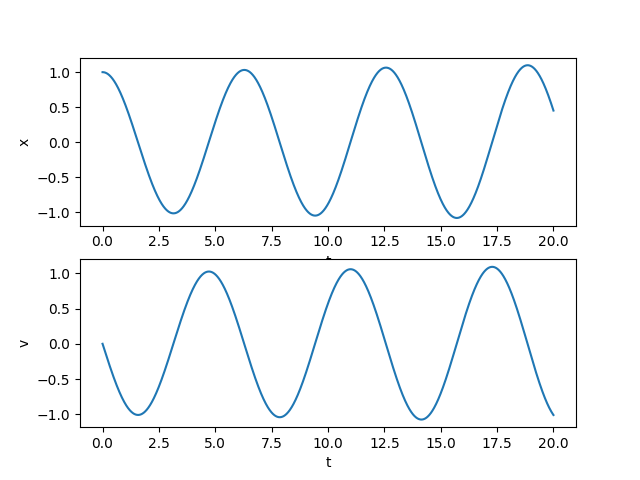
\includegraphics[scale=0.54]{x_and_v_plot_1_0_0-01_20.png}
\caption{Plot of $x$ and $v$ as functions of time for initial conditions $x(0) = 1$, $v(0) = 0$, and stepsize $h = 0.01$.}
\label{explicit}
\end{figure}
\newpage

2. We observe that the analytical solution to the simple harmonic oscillation equation $F = -kx$ for the intial conditions given is $x = \cos(t)$ and $v = -\sin(t)$.

We can compare our numerical solution to the analytic solution by plotting the global errors $x_{analytic}(t_i) - x_i$ and $v_{analytic}(t_i) - v_i$ against time.
\begin{figure}[htp]
\centering
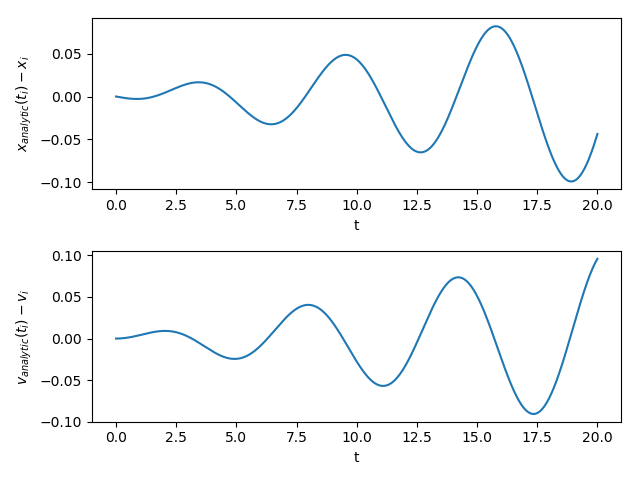
\includegraphics[scale=0.70]{x_err_and_v_err_plot_1_0_0-01_20.png}
\caption{Plot of global errors against time for the explicit Euler method, with stepsize $h=0.01$.}
\label{expliciterror}
\end{figure}
\newpage

3. We now plot the maximum global error in $x$ against $h$, integrating up to the same final time $t = 20$.
\begin{figure}[htp]
\centering
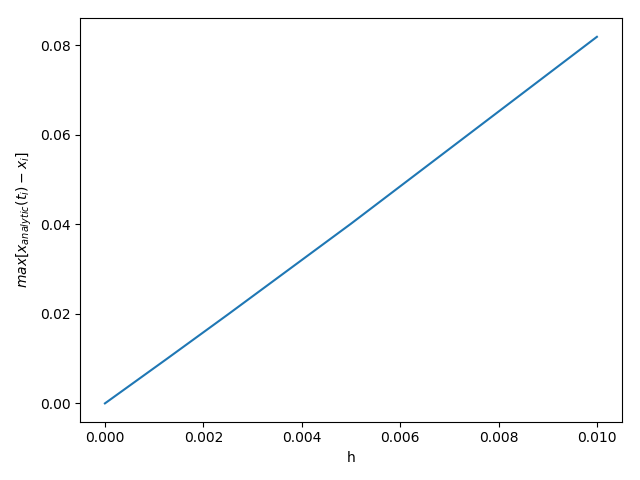
\includegraphics[scale=0.70]{err_behavior_0-01_4_20.png}
\caption{Plot of maximum global error in $x$ against $h$ for the explicit Euler method, integrating up to $t=20$ for each $h$.}
\label{expliciterrbehavior}
\end{figure}

The plot indicates that the truncation error is proportional to $h$ for reasonable $h$.
\newpage

4. We now plot the normalized total energy $E=v^2 + x^2$ as a function of time:
\begin{figure}[htp]
\centering
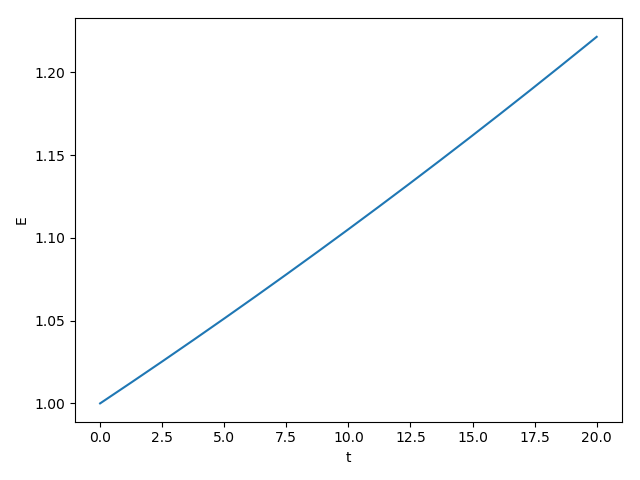
\includegraphics[scale=0.7]{energy_1_0_0-01_20.png}
\caption{Normalized energy computed from the results of the explicit Euler method for the same initial conditions and with $h=0.01$ as before.}
\label{eulerenergy}
\end{figure}

We observe that there is a linear increase with time of the normalized energy, similar to the behavior of the global error in with respect to h.

5. We implement the implicit Euler method using the recurrence relations:
\begin{align*}
x_i &= x_{i-1}+hv_{i-1} \\
v_i &= -x_{i-1}+v_{i-1}
\end{align*}
We then plot the global error behavior and the normalized energy as we did for our implementation of the explicit Euler method, making sure to use the same $h=0.01$ for the normalized energy plot to draw a fair comparison.
\newpage
\begin{figure}[htp]
\centering
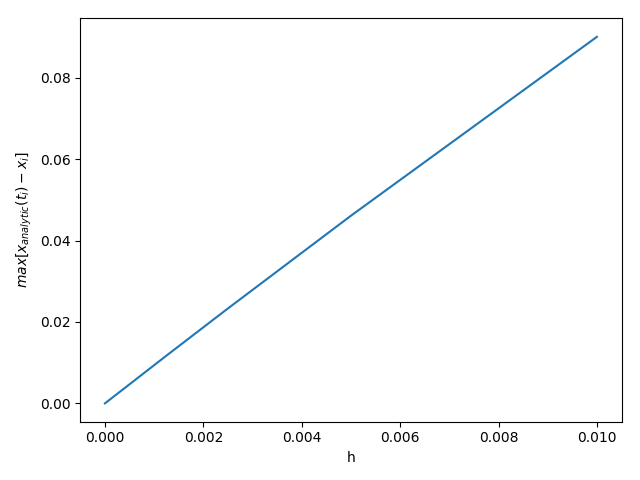
\includegraphics[scale=0.70]{implicit_err_behavior_0-01_4_20.png}
\caption{Plot of maximum global error in $x$ against $h$ for the implicit Euler method, integrating up to $t=20$ for each h.}
\label{impliciterr}
\end{figure}
We observe that the global error for the implicit Euler method behaves identically to the global error for the explicit Euler method.
\newpage

\begin{figure}[htp]
\centering
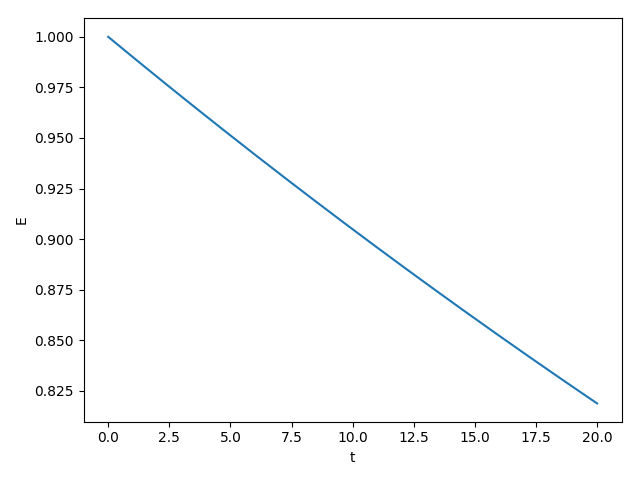
\includegraphics[scale=0.70]{implicit_energy_1_0_0-01_20.png}
\caption{Normalized energy computed from the results of the implicit Euler method for the same initial conditions and with $h=0.01$ as before.}
\label{implicitenergy}
\end{figure}
We observe that the normalized energy for the implicit Euler method decreases linearly in time, with gradient negative that for the explicit Euler method.
\newpage

\section*{Part 2}
1. We plot our solutions in phase space (plotting $v$ againsts $x$) setting $h=0.01$ and integrating up to $t=20$.

First, we do this for the analytical solution for the system:
\begin{figure}[htp]
\centering
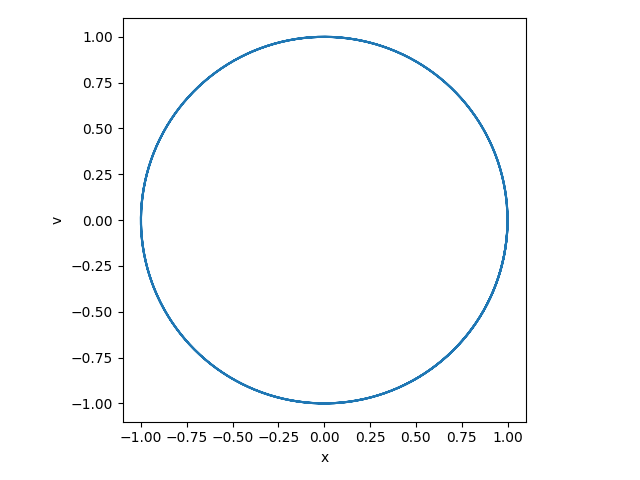
\includegraphics[scale=0.80]{analytic_phase_space_1_0_0-01_20.png}
\caption{Plotting the analytic solution in phase space, up to $t=20$.}
\label{analphase}
\end{figure}
\\
This solution is exactly what we would expect, since $E=x^2+v^2$ is conserved.
\newpage

We then plot the numerical solution obtained using the explicit Euler method:
\begin{figure}[htp]
\centering
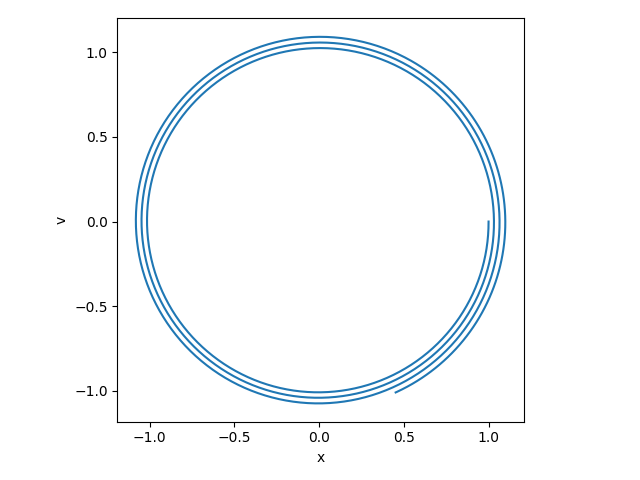
\includegraphics[scale=0.80]{euler_phase_space_1_0_0-01_20.png}
\caption{Plotting the numerical solution obtained using the explicit Euler method, integrating up to $t=20$.}
\label{eulphase}
\end{figure}
\\
This is what we expect for this method, since errors are induced such that $E$ increases linearly in time, i.e. trajectories in phase space spiral outwards.
\newpage

\begin{figure}[htp]
\centering
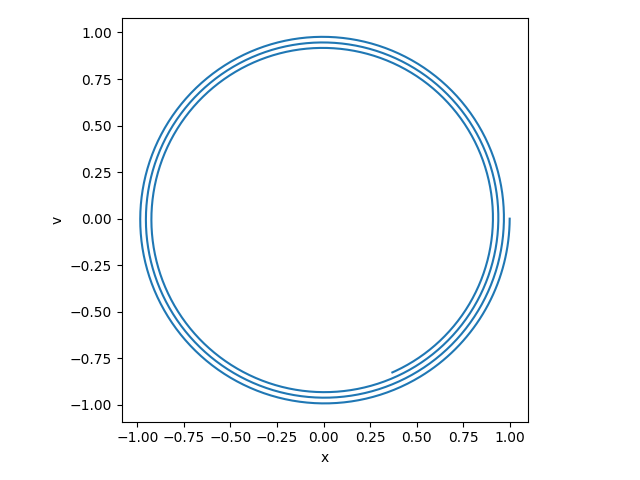
\includegraphics[scale=0.80]{implicit_euler_phase_space_1_0_0-01_20.png}
\caption{Plotting the numerical solution obtained using the implicit Euler method, integrating up to $t=20$.}
\label{impphase}
\end{figure}
This is what we expect for this method, since errors are induced such that $E$ increases linearly in time, i.e. trajectories in phase space spiral inwards.

2. We implement the symplectic Euler method, and again plot the numerical solution obained in phase space, setting $h=0.01$ and integrating up to $t=20$. \\
\newpage

\begin{figure}[htp]
\centering
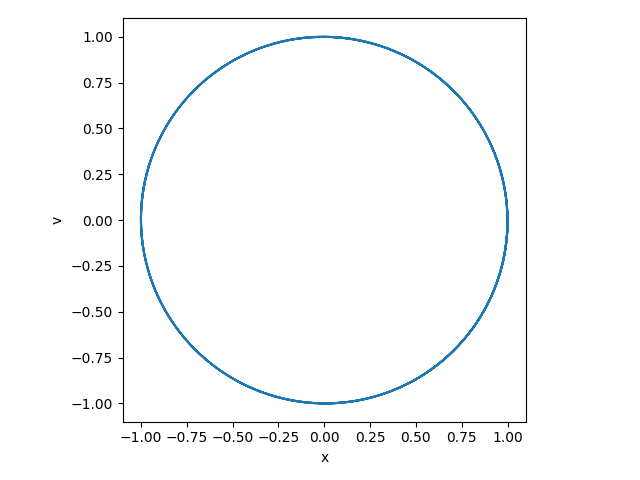
\includegraphics[scale=0.80]{symplectic_euler_phase_space_1_0_0-01_20.png}
\caption{Plotting the numerical solution obtained using the symplectic Euler method, integrating up to $t=20$.}
\label{sympphase}
\end{figure}

This shows the behavior we expect from a symplectic method in that it conserves $E$, i.e. the curve in phase space is closed and bounded.
\newpage

3. We now plot the evolution of $E=x^2+v^2$ with time, using the symplectic Euler method, setting $h=0.01$ and integrating to $t=20$. \\

\begin{figure}[htp]
\centering
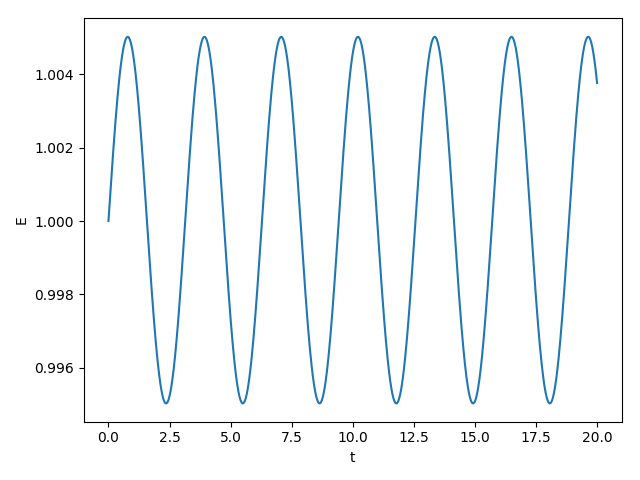
\includegraphics[scale=0.80]{symplectic_energy_1_0_0-01_20.png}
\caption{Normalized energy computed from the results of the symplectic Euler method for the same initial conditions and with $h=0.01$ as for all parts above, integrating up to $t=20$.}
\label{sympenergy}
\end{figure}

We first note that the analytic solution for $E$ with respect to time is obviously the line $E=1$ since $E$ is conserved. We can therefore observe that the deviations from $E=1$ time-average to zero, as we expect from a symplectic solution. This is exactly what we saw in phase space: there are slight deviations from a perfect circle but the resulting curve is nevertheless closed and encloses the same area as the analytic phase space curve, indicating that deviation time-average to zero.
\end{document}